% cdc.tex
% 
% author : abisutti
% created : Mon, 19 Oct 2015 13:48:21 +0200
% modified : Mon, 19 Oct 2015 13:48:21 +0200



\documentclass{beamer}

\usepackage[T1]{fontenc}
\usepackage[utf8]{inputenc}
\usepackage[francais]{babel}
\usepackage{array}
\usepackage{tabularx}
\usepackage{multirow}
\usepackage{color}
\usepackage{colortbl}
\usepackage{textcomp}
\usepackage{xstring}

%%% MACRO %%%


% FIXME Prendre en compte les majuscule déjà présente
\makeatletter
\@ifpackageloaded{xstring}{
	\newcommand\smallcaps[1]{\StrLeft{#1}{1}\scriptsize\uppercase{\StrGobbleLeft{#1}{1}}\normalsize }
}{
	\newcommand\smallcaps[1]{\textsc{#1}}
}
\makeatother



%===============================================================================
% Définit un type de puce pour une liste. Si le pakage "pifont" est chargé, il 
% est utilisé, sinon on met un tiret.
\makeatletter
\@ifpackageloaded{pifont}{
	\newcommand\goodItemArrow[0]{\ding{226}}
}{
	\newcommand\goodItemArrow[0]{-}
}
\makeatother



%===============================================================================
% Item de liste avec spécification de la puce et paramètre écrit en gras.
\newcommand\functionality[1]{
	\item[\goodItemArrow] \textbf{#1}\\
}



%===============================================================================
% Commande \Euro indépendante des paquets chargés 
\makeatletter
\@ifpackageloaded{eurosym}{
	\newcommand\Euro[0]{\euro{}}
}{
	\@ifpackageloaded{textcomp}{
		\newcommand\Euro[0]{\texteuro}
	}{
		\newcommand\Euro[0]{Euro}
	}
}
\makeatother



%===============================================================================
% Accès à des variables dans le document. 
%\makeatletter
%\let\titleName\@title
%\let\subtitleName\@subtitle
%\let\authorName\@author
%\makeatother



% Titre de la section courante (que dans beamer)
%\secname 
% Titre de la sous-section courante (que dans beamer)
%\subsecname





\title[R\'eunion de lancement]{Surfaces de r\'evolution discrètes}
\subtitle{R\'eunion de lancement}
\author[]{Zied \smallcaps{Ben} \smallcaps{Othmane} \\ Thomas \smallcaps{Benoist} \\ Adrien \smallcaps{Bisutti} \\ Lydie \smallcaps{Richaume}} % FIXME Enlever les parenthèses
\institute{Universit\'e de Poitiers}
\date{4 novembre 2015}

\usetheme{Madrid}
\usecolortheme{sidebartab}
\usefonttheme{professionalfonts}
%\useinnertheme{nom du theme interne}
%\useoutertheme{nom du theme externe}



%%% MACRO %%%

% Affichage du plan à chaque début de section
\AtBeginSection[]{
	\begin{frame}{Plan}
		\begin{columns}
			\begin{column}{5cm}
			  	\tableofcontents[sections={1-4}, currentsection, hideothersubsections]
			\end{column}
			\begin{column}{5cm}
			  	\tableofcontents[sections={5-7}, currentsection, hideothersubsections]
			\end{column}
		\end{columns}
	\end{frame}
}

% Nouvelle boîte pour le titre
\definecolor{titlecolor}{RGB}{51, 51, 179}
\newenvironment<>{titleblock}[1]{%
	\setbeamercolor{block body}{fg=white, bg=titlecolor}%
	\begin{block}#2{#1}}{\end{block}}

% Vide la barre de navigation
\setbeamertemplate{navigation symbols}{}

%%% DOCUMENT %%%

\begin{document}


%===============================================================================
%	TITRE
%===============================================================================


\begin{frame}
	\titlepage
	
\includegraphics[width=2cm]{../Images/logo-Xlim.png}
	\hfill
	
\includegraphics[width=2cm]{../Images/logo_univ_poitiers.png}
\end{frame}



%===============================================================================
%	PLAN
%===============================================================================


\begin{frame}{Plan}
	\begin{columns}
		\begin{column}{5cm}
			\tableofcontents[sections={1-4}, hideallsubsections]
		\end{column}
		\begin{column}{5cm}
			\tableofcontents[sections={5-7}, hideallsubsections]
		\end{column}
	\end{columns}
\end{frame}



%===============================================================================
%	INTRODUCTION
%===============================================================================

\section{Introduction}


% --- Équipe -------------------------------------------------------------------
	\subsection{Collaborateurs et clients}
	\begin{frame}{\subsecname}
		\begin{itemize}
			\item Clients~:
				\begin{itemize}
					\item \'Eric \smallcaps{Andres} (Professeur et ancien directeur de d\'epartement XLIM-SIC)
					\item Gaëlle \smallcaps{Largeteau}-\smallcaps{Skapin} (Maitre de Conf\'erence, G\'eom\'etrie~discr\`ete)
				\end{itemize}
			\item Exemple d'utilisateur final~:
				\begin{itemize}
					\item Aur\'elie \smallcaps{Mourier} (Artiste)
				\end{itemize}
			\item Encadrant p\'edagogique~: 
				\begin{itemize}
					\item Philippe \smallcaps{Meseure} (Professeur, Informatique graphique)
				\end{itemize}
		\end{itemize}
	\end{frame}


% --- Contexte -----------------------------------------------------------------
	\subsection{Contexte}
	\begin{frame}{\subsecname}
		\begin{itemize}
			\item Nouvel algorithme conçu par \'Eric \smallcaps{Andres} et Gaëlle \smallcaps{Largeteau}-\smallcaps{Skapin} pour mod\'eliser des surfaces de r\'evolution discrètes.
			\item Visualisation des r\'esultats avec Mathematica
		\end{itemize}
		\begin{figure}
			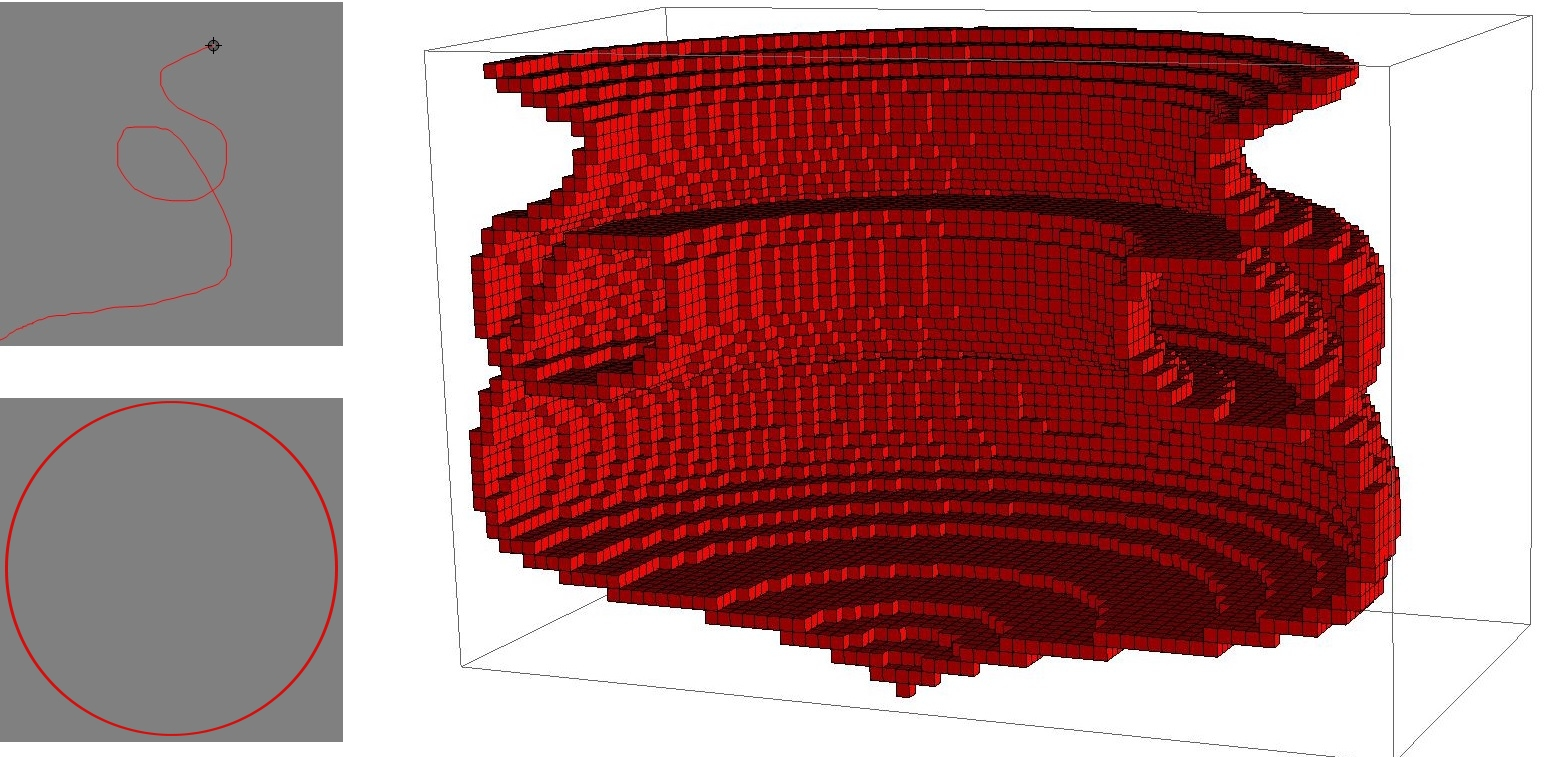
\includegraphics[height=3.8cm]{../Images/revolution2.jpg}
		\end{figure}
		\begin{itemize}
			\item Besoin d'un outil utilisable partout et par tous
		\end{itemize}
	\end{frame}
	


%===============================================================================
%	ORGANISATION
%===============================================================================

\section{Organisation de l'\'equipe}


% --- Roles --------------------------------------------------------------------
	 \subsection{Les r\^oles}
	 \begin{frame}{\subsecname}
		\begin{itemize}
			\item Composition de l'\'equipe~:
				\begin{itemize}
					\item Thomas \smallcaps{Benoist} - Chef de projet
					\item Zied \smallcaps{Ben} \smallcaps{Othmane} - Responsable qualit\'e
					\item Adrien \smallcaps{Bisutti} - Responsable des risques
					\item Lydie \smallcaps{Richaume} - Responsable des t\^aches
				\end{itemize}
		\end{itemize}
	\end{frame}


% --- Réunion ------------------------------------------------------------------
	\subsection{R\'eunions}
	\begin{frame}{\subsecname}
		\begin{itemize}
			\item R\'eunions de jalons :
			\begin{itemize}
				\item En pr\'esence des clients
				\item Première r\'eunion : aux environs du 20 d\'ecembre
				\item Possibilit\'e d'ajouter des r\'eunions durant le projet
			\end{itemize}
			\item Audits
			\begin{itemize}
				\item En pr\'esence de l'encadrant p\'edagogique, de l'auditeur et des clients
				\item R\'eunion de suivi, r\'eunion d'avancement, livraison, soutenance
			\end{itemize}
			\item R\'eunions avec l'encadrant p\'edagogique chaque semaine
		\end{itemize}
	\end{frame}



%===============================================================================
%	DEROULEMENT
%===============================================================================

\section{Planification}


% --- Taches -------------------------------------------------------------------
	\subsection{T\^aches}
	\begin{frame}{\subsecname}
		\begin{center}
		{\renewcommand{\arraystretch}{1.3}
		\begin{tabularx}{11cm}{|>{\hfill}X<{\hspace*{\fill}}|X<{\centering}|} % FIXME numéroté les tâches et faire voir les numéro le plus possibes !
			\hline
			\multicolumn{2}{|c|}{1 - Documentation, test et aide utilisateur}\\
			\hline
			\multicolumn{2}{|c|}{6 - Conception}\\
			\hline
			6 - Noyau fonctionnel & 10 - Interface minimale\\
			\hline
			17 - Ajout de fonctionnalités & \multirow{3}*{14, 22, 32 - Am\'elioration IHM}\\
			\cline{1-1}
			25 - M\'eridienne \`a main levée & \\%Am\'elioration IHM\\
			\cline{1-1}
			29 - Gestion des donn\'ees & \\%Am\'elioration IHM\\
			\hline
			\multicolumn{2}{|c|}{36 - Ajout courbe utilisateur}\\
			\hline
			\multicolumn{2}{|c|}{37 - R\'edaction rapport technique}\\
			\hline
		\end{tabularx}}
		\end{center}
	\end{frame}


% --- Pert ---------------------------------------------------------------------
	\subsection{Diagramme de Pert} % FIXME numéroté les tâches pour pouvoir utilisé cette numérotation
	\begin{frame}{Pert}
		\begin{figure}
			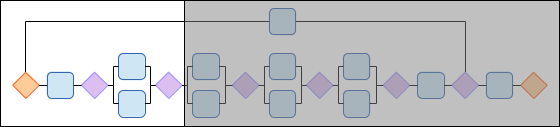
\includegraphics[width=6cm]{ImagesLancement/miniature1.png}
		\end{figure}\begin{figure}
			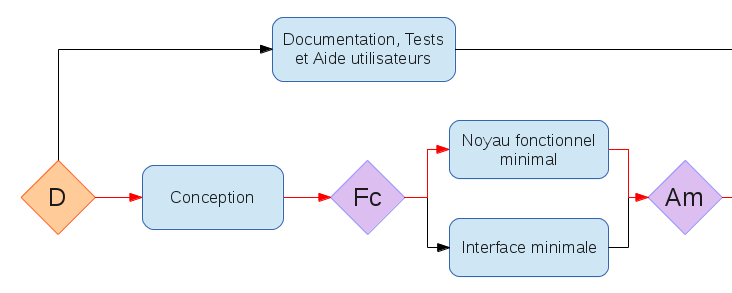
\includegraphics[width=11cm]{ImagesLancement/pert_part_1.png}
		\end{figure}
		\footnotesize{D~: D\'epart (30/10) \hfill Am~: Appli. minimale (24/12) \\
			\hfill Fc~: Fin conception (16/12) \hspace*{\fill}}
	\end{frame}

	\begin{frame}{Pert}
		\begin{figure}
			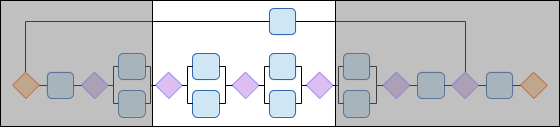
\includegraphics[width=6cm]{ImagesLancement/miniature2.png}
		\end{figure}\begin{figure}
			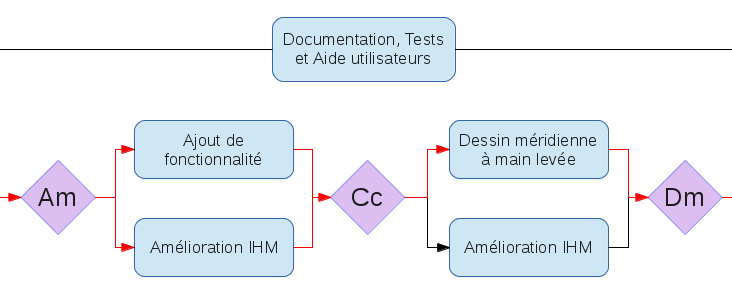
\includegraphics[width=11cm]{ImagesLancement/pert_part_2.png}
		\end{figure}
		\footnotesize{Am~: Appli. minimale (24/12) \hfill Dm~: Dessin main lev\'ee (28/01)\\
			 \hfill Cc~: Choix des courbes (20/01) \hspace*{\fill}}
	\end{frame}

	\begin{frame}{Pert}
		\begin{figure}
			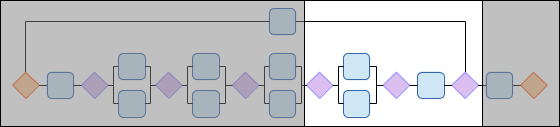
\includegraphics[width=6cm]{ImagesLancement/miniature3.png}
		\end{figure}\begin{figure}
			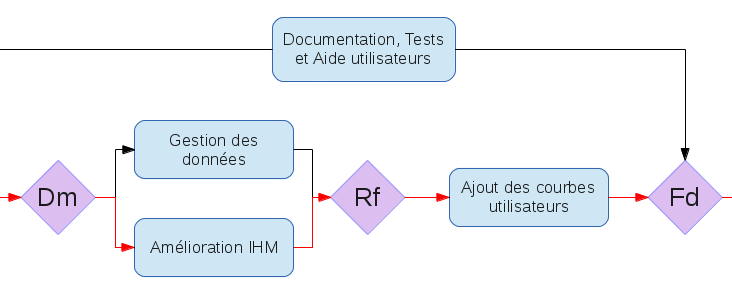
\includegraphics[width=11cm]{ImagesLancement/pert_part_3.png}
		\end{figure}
		\footnotesize{Dm~: Dessin main lev\'ee (28/01) \hfill Fd~: Fin d\'eveloppement (02/03)\\
			 \hfill Rf~: Rentrer formule (19/02)\hspace*{\fill}}
	\end{frame}

	\begin{frame}{Pert}
		\begin{figure}
			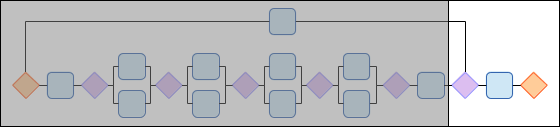
\includegraphics[width=6cm]{ImagesLancement/miniature4.png}
		\end{figure}\begin{figure}
			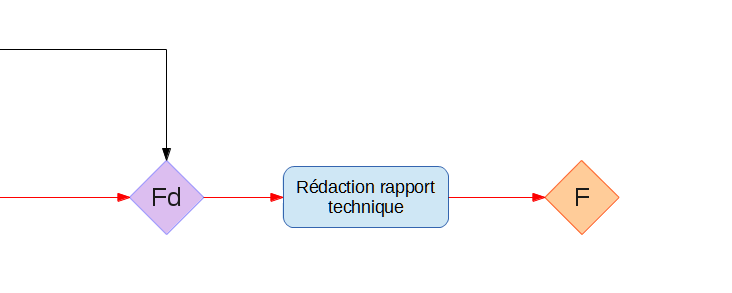
\includegraphics[width=11cm]{ImagesLancement/pert_part_4.png}
		\end{figure}
		\footnotesize{Fd~: Fin d\'eveloppement (02/03) \hfill F~: Fin (17/03)\\[0.48cm]}
	\end{frame}
	

% --- Gantt --------------------------------------------------------------------
	\subsection{Diagramme de Gantt}
	\begin{frame}{Gantt}
		\begin{figure}
			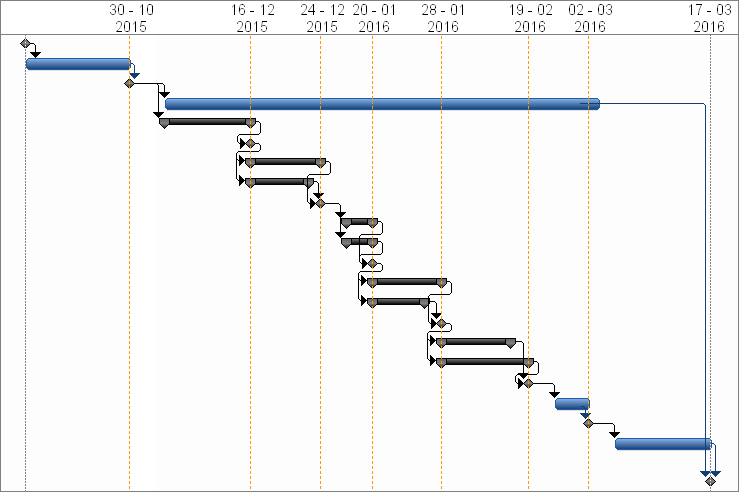
\includegraphics[height=7.5cm]{../Images/Gantt_Macro2.png} % FIXME mettre les tâches (nom et/ou numérotation) près des bandes
		\end{figure}
	\end{frame}


	\begin{frame}{Gantt}
		\begin{figure}
			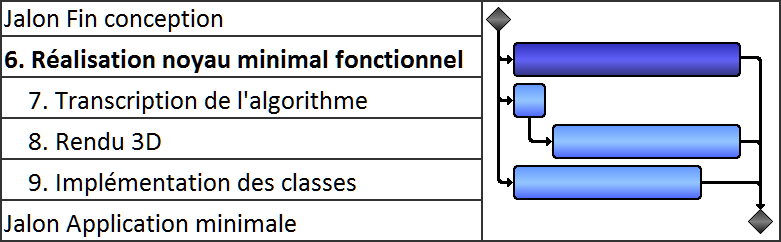
\includegraphics[width=12cm]{../Images/gantt_zoom_noyau.png} % FIXME modifié nom jalon
		\end{figure}
	\end{frame}


% --- Avancement ---------------------------------------------------------------
	\subsection{Avancement}
	\begin{frame}{\subsecname}
		\begin{figure}
			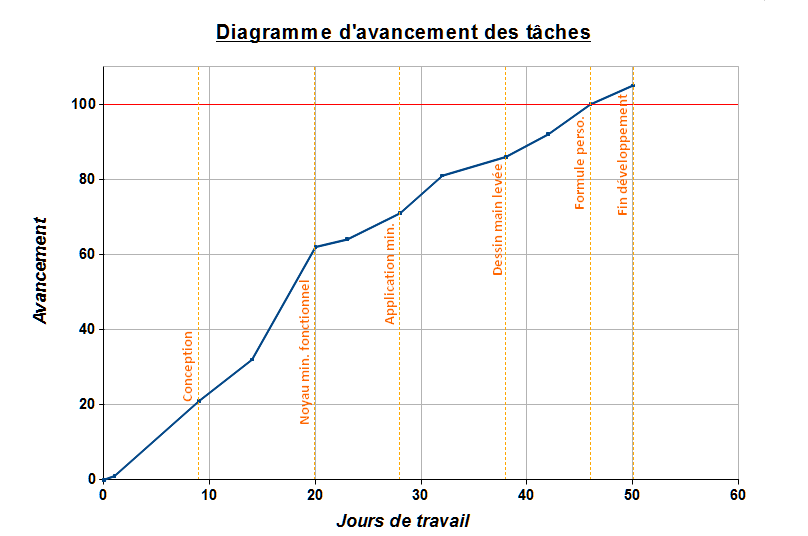
\includegraphics[width=12cm]{ImagesLancement/Avancement.png} % FIXME bien régler les points et faire apparaitre le livrables
		\end{figure}
	\end{frame}


% --- Livrables ----------------------------------------------------------------
	\subsection{Livrables}
	\begin{frame}{\subsecname}
		\begin{center}
		{\renewcommand{\arraystretch}{1.2}
		\begin{tabular}{|c|m{6.5cm}|c|} % FIXME relié les livrables au tâches
			\hline
			\textbf{\No} & \textbf{Livrable} & \textbf{Date pr\'evue}\\
			\hline
			1 & R\'esultat de l'algorithme et interface & 23/12\\
			\hline
			2 & Application minimale & 21/01\\
			\hline
			3 & Courbes avec paramètres modifiables et trac\'e \`a main lev\'ee & 29/01\\
			\hline
			4 & \'Equations et export & 19/02\\
			\hline
			5 & Application finale et documentation & 02/03\\
			\hline
		\end{tabular}}
		\end{center}
		Types de livrables~:
		\begin{itemize}
			\item Version logicielle~: tous
			\item Documentation utilisateur~: tous
			\item Documentation technique~: 1 et 5
		\end{itemize}
	\end{frame}



%===============================================================================
%	RISQUES
%===============================================================================

\section{Risques}


% --- Risques ------------------------------------------------------------------
	\subsection{Risques sp\'ecifiques}
	\begin{frame}{\subsecname}
		Liste non exhaustive des risques identifi\'es~:
			\begin{itemize}
				\item \'Evolution de l'algorithme de g\'en\'eration (criticit\'e~: 2)
				\item Transcription de l'algorithme difficile (Mathematica $\to$ Javascript) (1)
				\item Interface \`a r\'ealiser pour deux cat\'egories d'utilisateurs (1)
				\item Rendu 3D demandant trop de ressources (1)
				\item Problèmes li\'es au serveur (0)
			\end{itemize}
	\end{frame}

% FIXME ne pas oublier les solution (préventives et curatives) au moins à l'oral
	\begin{frame}{\subsecname}
		\begin{itemize}
			\item \'Evolution de l'algorithme de g\'en\'eration
		\end{itemize}
		\begin{figure}
			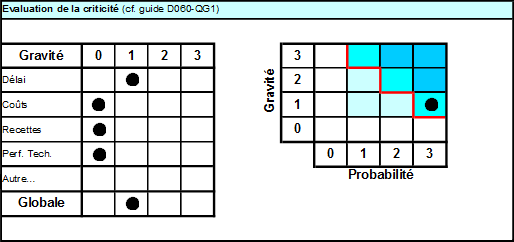
\includegraphics[width=8cm]{ImagesLancement/Evolution_algo.png}
		\end{figure}
		\begin{figure}
			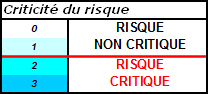
\includegraphics[height=2cm]{ImagesLancement/legende_risque2.png} % FIXME compléter avec légende gravité et probabilité
		\end{figure}
	\end{frame}

	\begin{frame}{\subsecname}
		\begin{itemize}
			\item Interface \`a r\'ealiser pour deux cat\'egories d'utilisateurs
		\end{itemize}
		\begin{figure}
			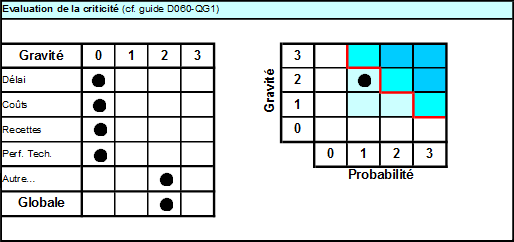
\includegraphics[width=8cm]{ImagesLancement/Interface_2_user.png}
		\end{figure}
		\begin{figure}
			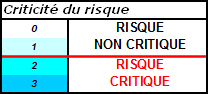
\includegraphics[height=2cm]{ImagesLancement/legende_risque2.png} % FIXME compléter avec légende gravité et probabilité
		\end{figure}
	\end{frame}


	\begin{frame}{\subsecname}
		\begin{itemize}
			\item Probl\`emes li\'es aux serveurs
		\end{itemize}
		\begin{figure}
			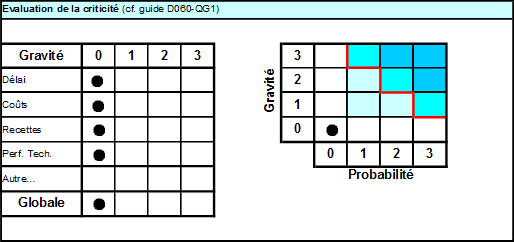
\includegraphics[width=8cm]{ImagesLancement/Serveur.png}
		\end{figure}
		\begin{figure}
			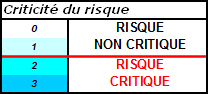
\includegraphics[height=2cm]{ImagesLancement/legende_risque2.png} % FIXME compléter avec légende gravité et probabilité
		\end{figure}
	\end{frame}


% --- Risques génériques -------------------------------------------------------
	\subsection{Risques g\'en\'eriques}
	\begin{frame}{\subsecname}
		\begin{itemize}
			\item Nouveaux clients (criticit\'e~: 1)
			\item Non respect du cahier des charges (1)
			\item Non ad\'equation d'un outil pr\'evu (1)
			\item Communication interne insuffisante (1)
		\end{itemize}
	\end{frame}



%===============================================================================
%	MISE EN OEUVRE ÉQUIPE
%===============================================================================

\section{M\'ethodologie}


% --- Mise en oeuvre -----------------------------------------------------------
	\subsection{Mise en \oe uvre}
	\begin{frame}{\subsecname}
		\begin{itemize}
			\item D\'eveloppement en spirale
				\begin{itemize}
					\item Un livrable \`a chaque fin de cycle (version de l'application et documentation correspondante)
					\item Documentation et tests durant chaque cycle
					\item Adaptation aux demandes des clients
					\item Six cycles \`a dur\'ee variable
				\end{itemize}
		\end{itemize}
		\begin{itemize}
			\item \'Evaluation de la qualit\'e logiciel
				\begin{itemize}
					\item PQL~: norme ISO-9126
					\item Attribution d'une note qualit\'e selon diff\'erents critères
					\item Tests internes et externes
				\end{itemize}
		\end{itemize}
	\end{frame}


% --- Tests --------------------------------------------------------------------
	\subsection{Tests}
	\begin{frame}{\subsecname}
		\begin{block}{Tests internes}
			\begin{itemize}
				\item Mesure de la qualit\'e du code de l'application
				\item Plans de tests d\'efinis par le responsable qualit\'e
				\item Tests unitaires effectu\'es par les d\'eveloppeurs de la classe
				\item Tests d'int\'egration effectu\'es par le responsable qualit\'e
			\end{itemize}
		\end{block}

		\begin{block}{Tests externes}
			\begin{itemize}
				\item Validation de l'application par les clients et le responsable qualité
				\begin{itemize}
					\item Validation des fonctionnalit\'es
					\item Validation de l'interface
				\end{itemize}
				\item Sc\'enarii de test sous forme de questionnaires aux clients
			\end{itemize}
		\end{block}
	\end{frame}


% --- Tests --------------------------------------------------------------------
	\subsection{Plan qualit\'e logiciel}
	\begin{frame}{\subsecname}
		\begin{figure}
			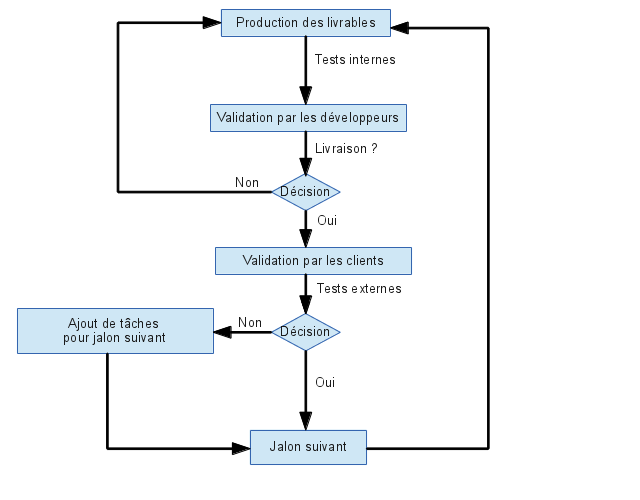
\includegraphics[height=8cm]{ImagesLancement/PAQL.png} % FIXME regénéré pour être plus lisible et spécifié "validation par les clients à chaque jalon"
		\end{figure}
	\end{frame}



%===============================================================================
%	COUTS
%===============================================================================

\section{Coûts}


\begin{frame}{\secname}
	\begin{itemize}
		\item Co\^ut total~:
			\begin{itemize}
				\item Jeune ing\'enieur~: 3 000 \Euro{} / mois
				\item 4 personnes pendant 10 semaines
				\item Co\^ut de revient~: 30 000 \Euro 
				\item Prix propos\'e~: 40 000 \Euro
			\end{itemize}
	\end{itemize}
	\begin{itemize}
		\item \'Etalement des paiements~:
			\begin{itemize}
				\item 30\% \`a la signature du cahier des charges (soit 12 000 \Euro)
				\item 10\% pour chaque livrable (soit 4 000 \Euro)
				\item 30\% \`a la livraison de l'application finale
			\end{itemize}
	\end{itemize}
\end{frame}


\begin{frame}{\secname}
	\begin{figure}
		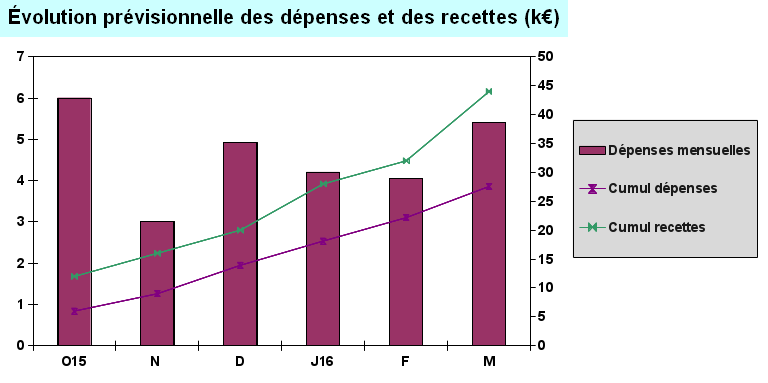
\includegraphics[width=12cm]{ImagesLancement/Cout2.png} % XXX voir ce que ça donne en semaine
	\end{figure}
\end{frame}



%===============================================================================
%	CONCLUSION
%===============================================================================

\section{Conclusion}


% --- Rappel -------------------------------------------------------------------
\begin{frame}{\secname}
	\begin{itemize}
		\item Organisation en cycles $\to$ d\'eveloppement incr\'emental
		\item Validation r\'egulière et avec les clients
		\item Un seul risque majeur
		\item Prochaine \'etape~: Conception
	\end{itemize}
\end{frame}


% --- Remerciment --------------------------------------------------------------
\begin{frame}{}
	\bigskip
	\bigskip
	\begin{titleblock}{}
		\begin{center}
			\smallskip
			\Large Surfaces de r\'evolution discrètes\\
			\medskip
			\small R\'eunion de lancement
			\smallskip
		\end{center}
	\end{titleblock}

	\bigskip
	\begin{center}
		Merci de votre attention.\\
		\medskip
		Avez-vous des questions\,?			
	\end{center}

	\bigskip
	\bigskip
	
\includegraphics[width=2cm]{../Images/logo-Xlim.png}
	\hfill
	
\includegraphics[width=2cm]{../Images/logo_univ_poitiers.png}
\end{frame}


\end{document}


